\section{Durchführung}
%Im Versuch werden mehrere Brückenschaltungen nach Schaltplan aufgebaut und die Nullmethode angewendet. Sobald die Spannung minimiert wurde, werden 
%die Widerstände $R_2$, $R_3$ und $R_4$ notiert. Diese Methode wird nacheinander auf die Wheatstonesche Brückenschaltung (), die Kapazitätsmessbrücke (Schaltplan in Abbildung (\ref{})) und die Induktivitätsmessbrücke (Schaltplan 
%in Abbildung (\ref{})) angewandt. Dabei sind bei jeder dieser Messbrücken zwei verschiedene, unbekannte Bauteile durch die Nullmethode zu bestimmen. Für jedes
%zu bestimmende Bauteil wird die Nullmethode 3 Mal mit verschiedenen Widerständen $R_2$ (und verschiedenen $C_2$ bei der Kapazitätsmessbrücke bzw. $L_2$ bei der
%Induktivitätsmessbrücke)
%
%Schaltplan in Abbildung (\ref{pic:Wheatstonesche_Brückenschaltung}) aufgebaut und die 
\subsection{Wheatstonesche Brücke}
Zuerst wird die Wheatstonesche Brückenschaltung nach Schaltplan in Abbildung (\ref{pic:Wheatstonesche_Brueckenschaltung}) aufgebaut. $R_3$ ist dabei ein Potentiometer
und $R_4$ ist durch $R_4 = 1000 \, \unit{\ohm} - R_3 $ festgelegt. Dann wird die Nullmethode angewendet.
Sobald die Spannung das Minimum erreicht, werden die Widerstände notiert. Diese Nullmethode wird insgesamt 3 Mal für einen unbekannten Widerstand angewendet, jeweils
mit unterschiedlichen $R_2$. Es werden zwei verschiedene unbekannte ohmsche Widerstände auf diese Weise bestimmt.  
\begin{figure}[H]
    \centering
    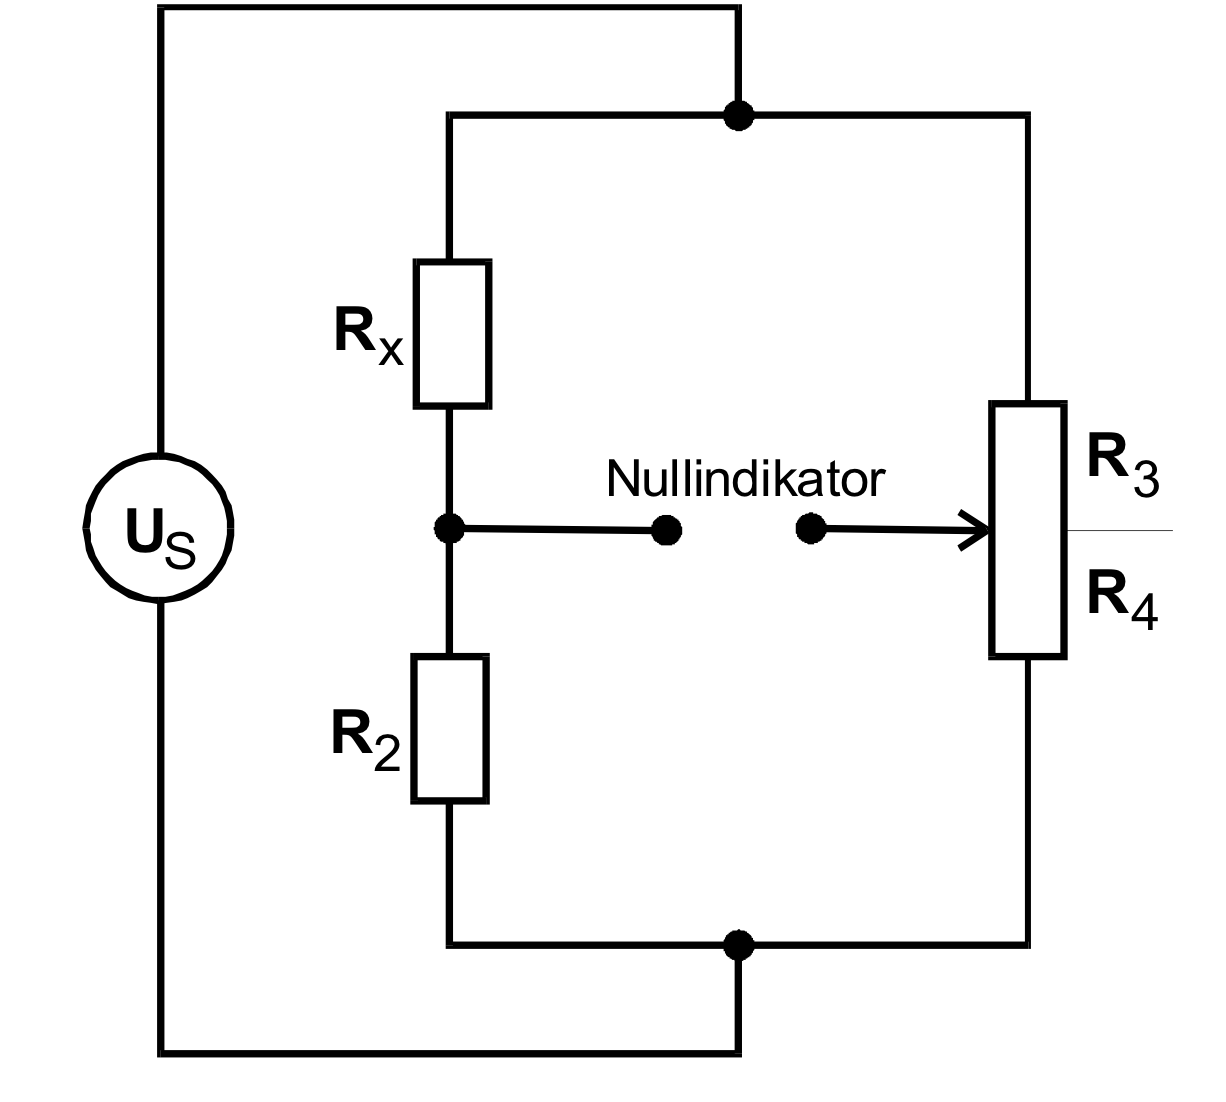
\includegraphics[width=0.4\linewidth]{Wheatstonesche.png}
    \caption{Schaltplan der Wheatstoneschen Brückenschaltung. Q\cite{anleitungV302}}
    \label{pic:Wheatstonesche_Brueckenschaltung}
\end{figure}
\subsection{Kapazitätsmessbrücke}
Die Kapazitätsmessbrücke wird nach Schaltplan in Abbildung (\ref{pic:Kapazitaetsmessbruecke}) aufgebaut und für $R_3$ bzw. $R_4$ wird dasselbe Potentiometer
verwendet wie bei der Wheatstoneschen Brücke. In diesem Teil des Versuches werden ebenfalls zwei unterschiedliche unbekannte Kapazitäten und zugehörige 
ohmsche Widerstände bestimmt durch je drei Messwerte. Bei jedem dieser Messwerte wird der Kondensator mit Kapazität $C_2$ und $R_2$ variiert, dann die Nullmethode durchgeführt und alle Kenngrößen
der bekannten Bauteile notiert. 
\begin{figure}[H]
    \centering
    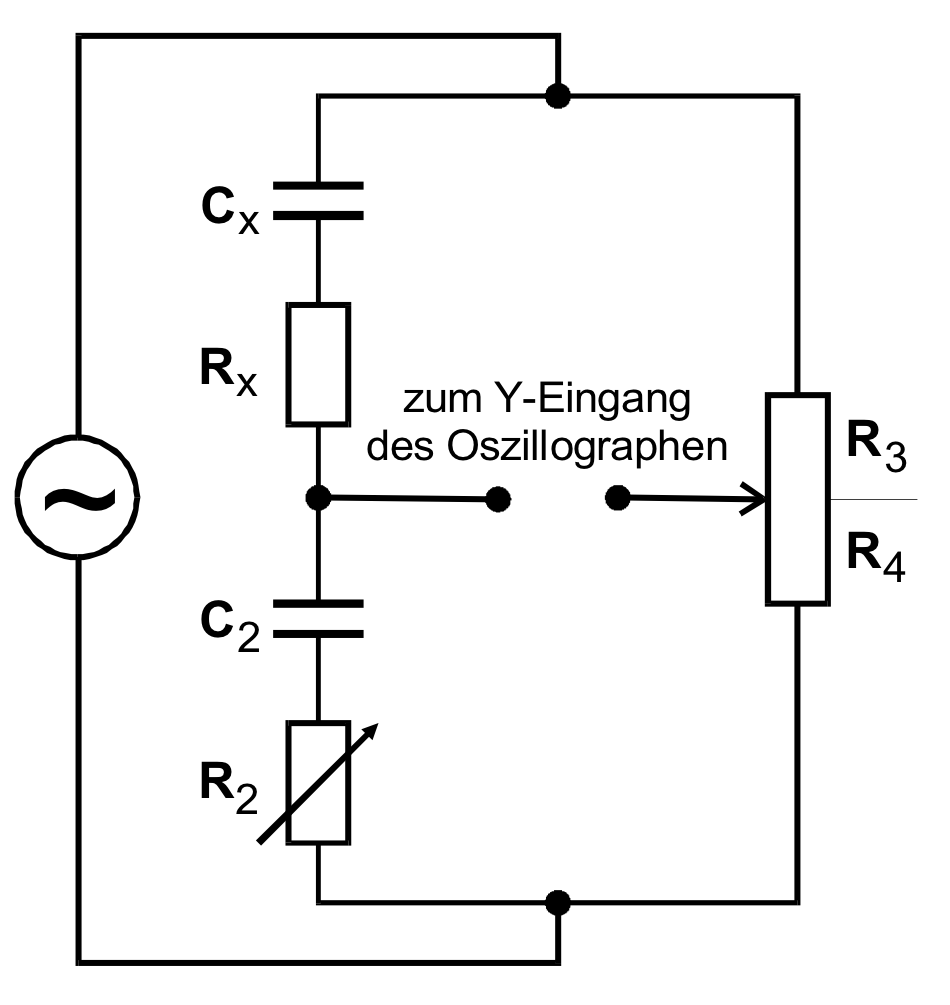
\includegraphics[width=0.4\linewidth]{Kapazitaet.png}
    \caption{Schaltplan der Kapazitätsmessbrücke. Q\cite{anleitungV302}}
    \label{pic:Kapazitaetsmessbruecke}
\end{figure}
\subsection{Induktivitätsmessbrücke}
Zur Messung zweier unbekannter Induktivitäten $L_x$ mit zugehörigem ohmschen Widerstand $R_x$ wird die Induktivitätsmessbrücke nach Schaltplan in Abbildung 
(\ref{pic:Induktivitaetsmessbruecke}) aufgebaut. Es werden die Kennzahlen zweier unterschiedlicher, unbekannter Spulen bestimmt, jeweils durch drei Messwerte bei 
denen $L_2$ und $R_2$ variiert wird. Zur Bestimmung von $R_3$ bzw. $R_4$ wird die Nullmethode angewandt und diese Widerstände notiert. 
\begin{figure}[H]
    \centering
    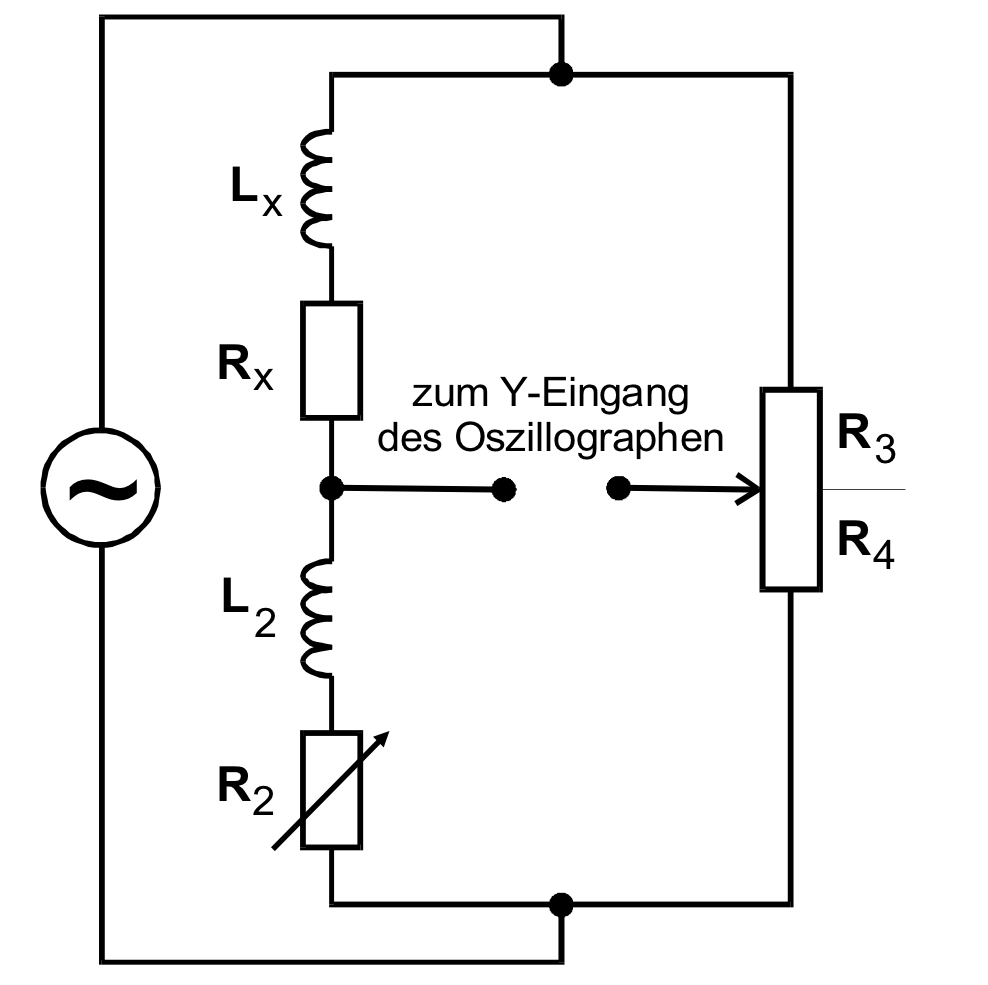
\includegraphics[width=0.4\linewidth]{Induktivitaet.png}
    \caption{Schaltplan der Induktivitätsmessbrücke. Q\cite{anleitungV302}}
    \label{pic:Induktivitaetsmessbruecke}
\end{figure} 
\subsection{Maxwell-Brücke}
Im folgenden Versuchsteil werden (idealerweise dieselben) zwei Induktivitäten $L_x$ mit zugehörigem ohmschen Widerstand $R_x$ erneut bestimmt mithilfe der 
Maxwell-Brücke. Der Schaltplan dieser Brücke ist in Abbildung (\ref{pic:Maxwell-Bruecke}) zu sehen. In diesem Versuchsteil sind $R_3$ und $R_4$ voneinander unabhängige
Potentiometer. Diese werden abwechselnd variiert bis das Spannungsminimum erreicht ist. Daraufhin werden alle Kennzahlen der Bauteile notiert. 
\begin{figure}[H]
    \centering
    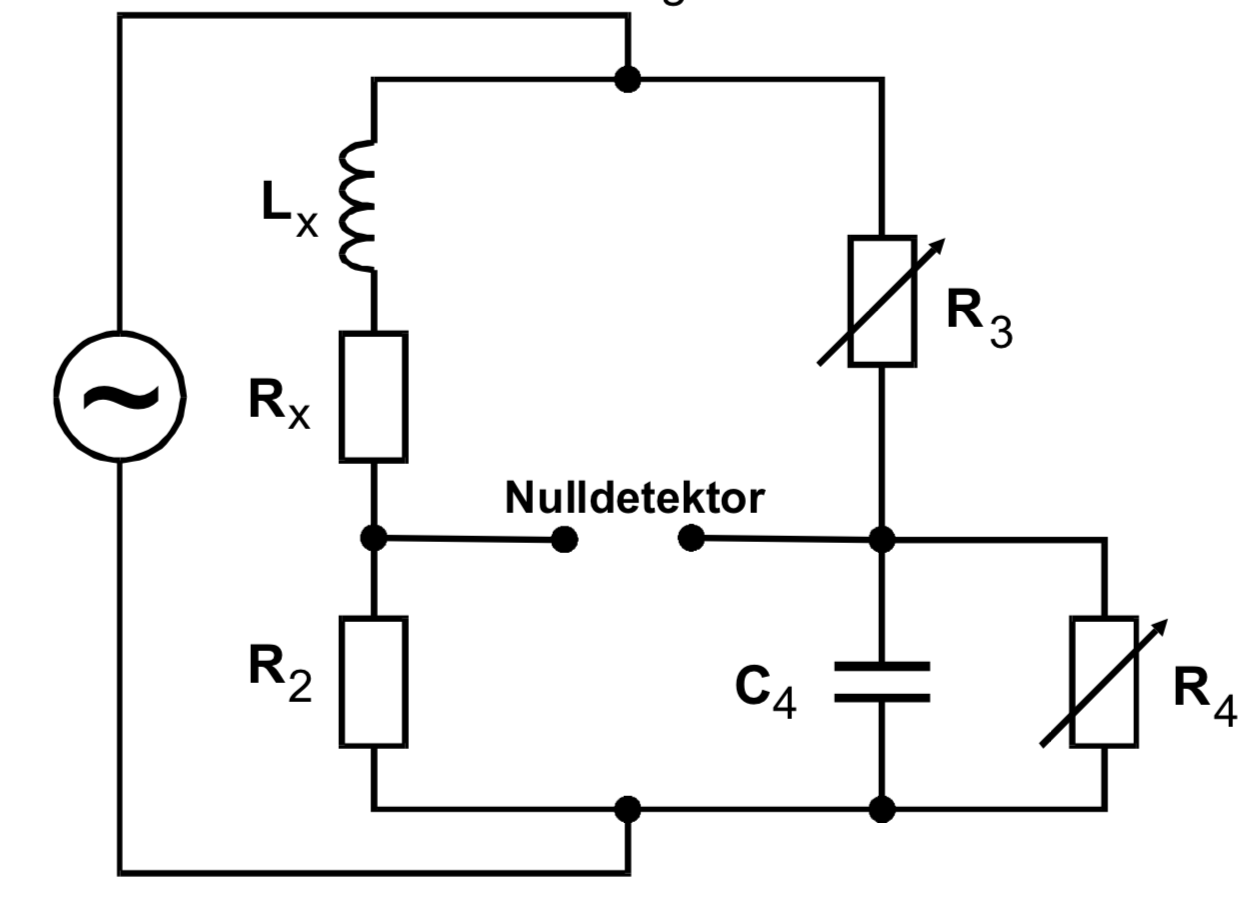
\includegraphics[width=0.4\linewidth]{Maxwell_Bruecke.png}
    \caption{Schaltplan der Maxwell-Brücke. Q\cite{anleitungV302}}
    \label{pic:Maxwell-Bruecke}
\end{figure} 
\subsection{Wien-Robinson-Brücke}
Die Wien-Robinson-Brücke wird gemäß Schaltplan in Abbildung (\ref{pic:WRB}) aufgebaut und für $R$ bzw. $R$' werden nur bekannte Widerstände verwendet. 
In diesem Teil des Versuchs wird die Frequenz der Quelle variiert und die resultierende Frequenz der Brückenspannung notiert. Im Bereich von 0 bis 500 Hz der Quellspannung 
werden die Messwerte in 50 Hz Schritten aufgenommen, von 500 bis 5000 Hz in 500 Hz Schritten. 
\begin{figure}[H]
    \centering
    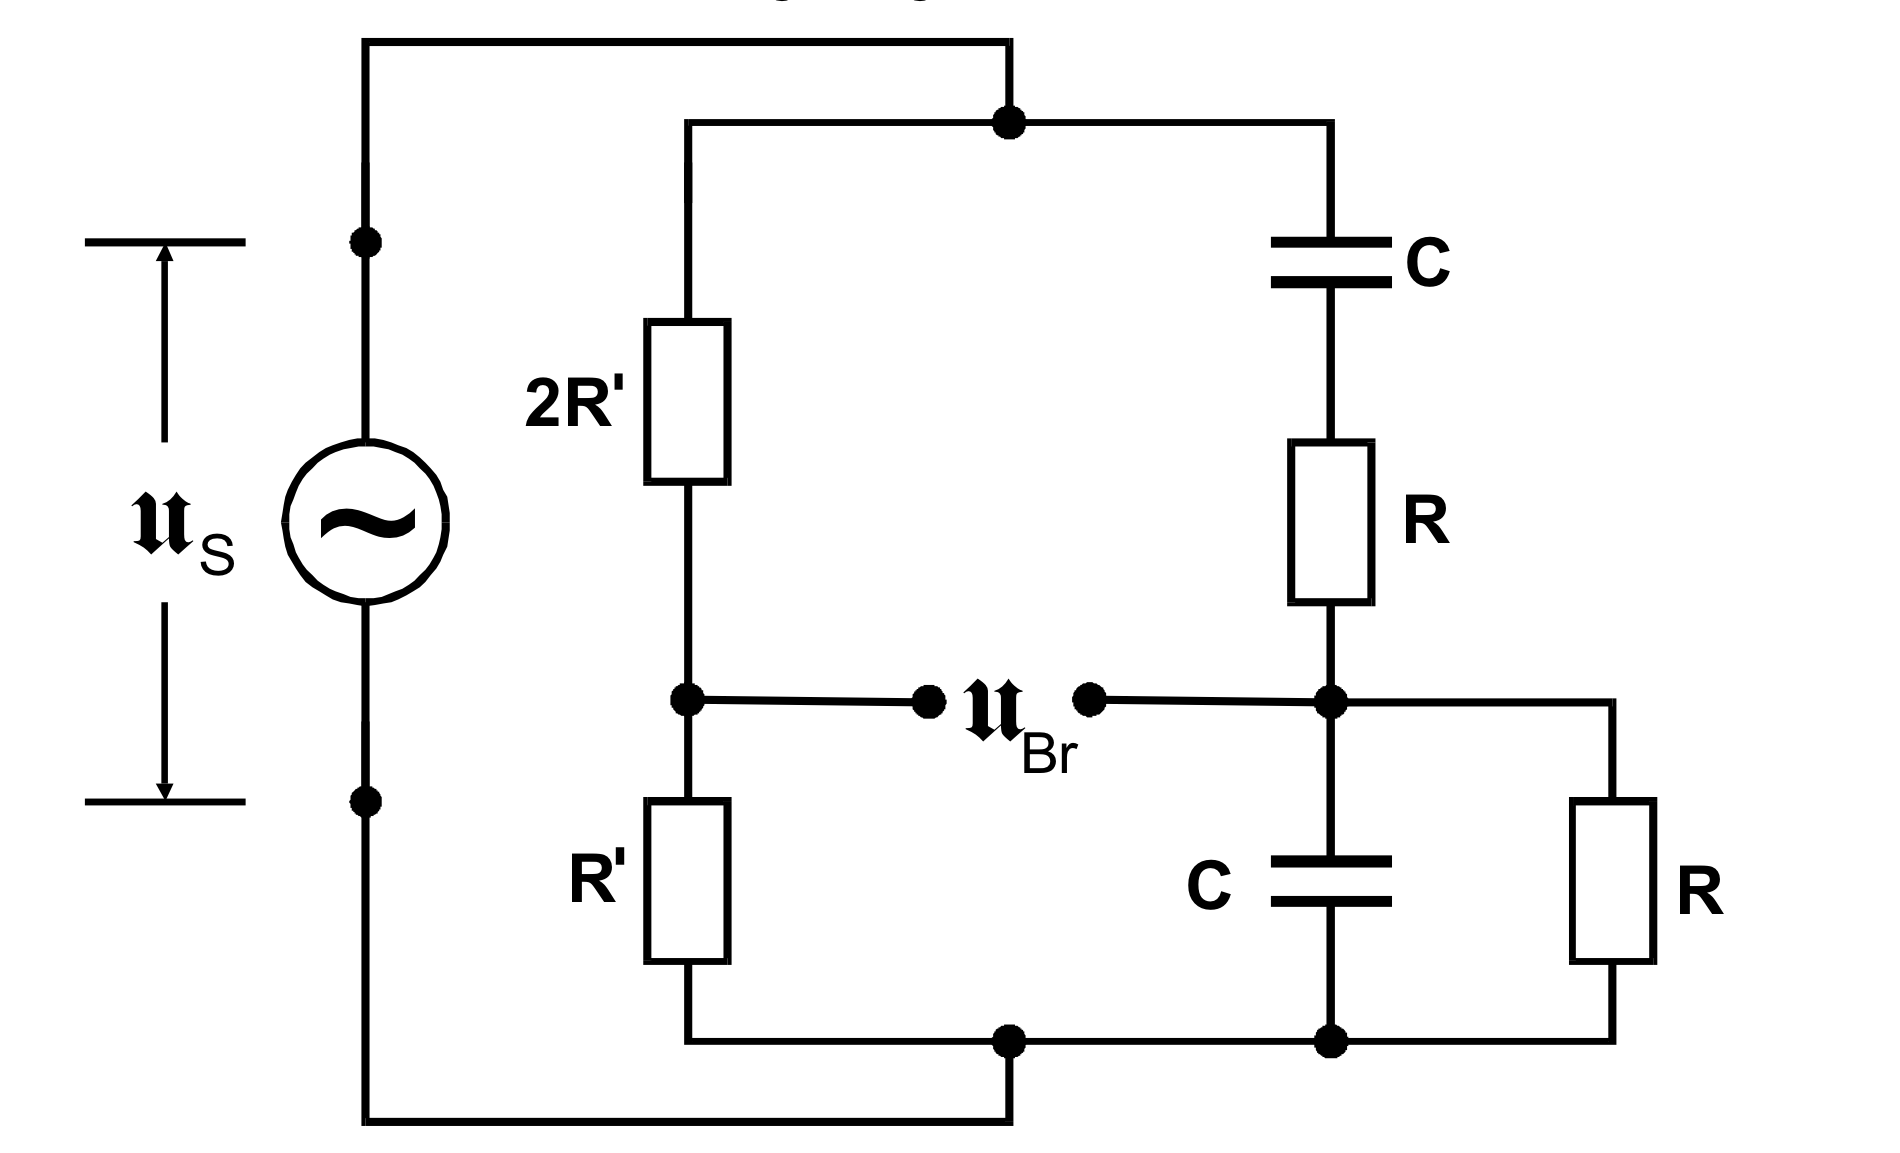
\includegraphics[width=0.4\linewidth]{Wienrobinson_Bruecke.png}
    \caption{Schaltplan der Wien-Robinson-Brücke. Q\cite{anleitungV302}}
    \label{pic:WRB}
\end{figure} 
%\subsection{Kirrfaktor}
%Der Klirrfaktor wird im Anschluss an den experimentellen Teil zur Qualitätseinschätzung des Oszilloskops bestimmt. 